\documentclass[a4paper]{scrartcl}

% Localization
\usepackage[english]{babel}
\usepackage[T1]{fontenc}
\usepackage[utf8]{inputenc}

% Quotations
\usepackage{dirtytalk}

% PDF-compatible landscape mode
\usepackage{pdflscape}

% Advanced tables
\usepackage{array}
\usepackage{tabularx}

% Fancy tablerules
\usepackage{booktabs}

% Graphics
\usepackage{caption}
\usepackage{subcaption}
\usepackage{graphicx}
\graphicspath{{resources}}

% Decent quotations
\usepackage{csquotes}

% Automatic float barriers to each \section
% \usepackage[section]{placeins}

% Math
\usepackage{amssymb,amsmath,amsfonts}
\usepackage{mathtools}

% Algorithms
\usepackage{algpseudocode}

% SI units
\usepackage[binary-units]{siunitx}

% Clickable links in PDF
\usepackage{hyperref}

\title{33107 - Document Image Processing}
\subtitle{Summary}
\author{Michael Senn}
\date{\today}

\begin{document}

\maketitle % Inserts the title, author and date

\tableofcontents

\begin{abstract}
		This summary is based on the lecture notes and slides. It was created
		for the sole purpose of preparing for an exam, with no focus on
		proof-reading, a coherent structure or being suitable for other people.
		Use at your own discretion.
\end{abstract}

% No summary for lecture 1 (introduction)
\setcounter{section}{1}

\section{Image Processing}

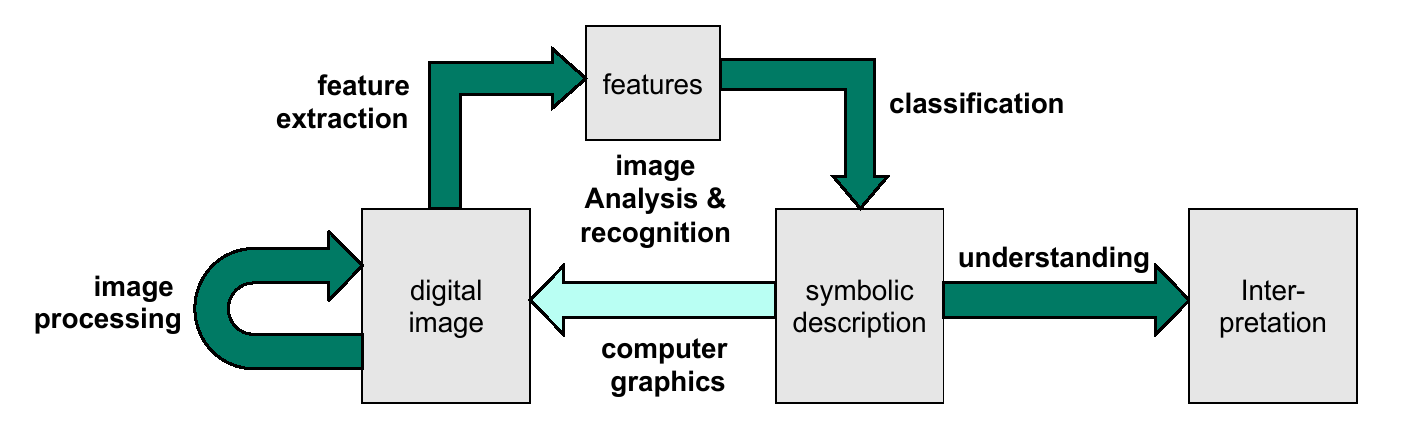
\includegraphics[width=\textwidth]{02_image_disciplines}

\begin{description}
		\item[Image digitalization] Sample to produces pixels, quantize to determine pixel values
		\item[Representation of digital image] Usually as 2D grid.
				Alternatively: Pyramid, with each layer a different resolution.
		\item[Color modes] Direct colour (channels) vs indexed colour (colour map)
		\item[Color spaces] Many different ones
		\item[Quantization] Determine range of pixel values
\end{description}


\subsection{Compression}

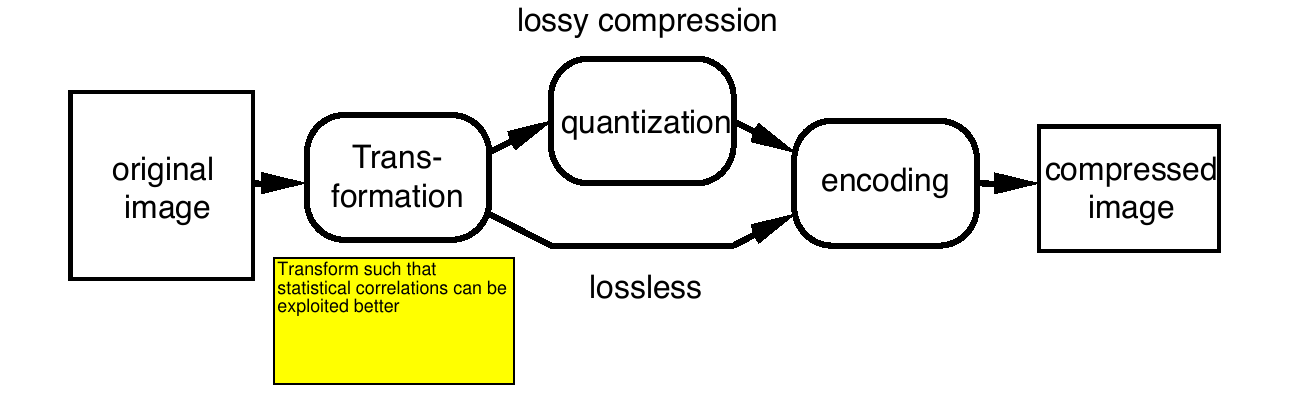
\includegraphics[width=\textwidth]{02_compression}

\begin{itemize}
		\item Lossy vs lossless
		\item Entropy $H(x) = - \sum_{i=1}^n p(i) \log_2(p(i))$. Maximal $H(x)
				= \log_2(n)$ iff all states equally likely (eg uniform noise).
				Minimal $H(x) = 0$ if only one state.
		\item Example: Huffman code, quadtree (recursively partition into four
				quadrants until you get homogenous space)
\end{itemize}

\subsection{Processing operations}

\begin{description}
		\item[Point operation] $z = f(u)$, output depends only on corresponding
				pixel of input. Eg colour inversion, threshold, logical
				combinations.
		\item[Local operation] Each output pixel $(x, y)$ depends on
				neighbourhood $V(x, y)$ of source. Eg convolution operations,
				morphological filters, statistical filters.
		\item[Global operation] Output pixel depends on all pixels of source.
\end{description}

\subsubsection{Convolution}

Mathematical operation of two functions $f$, $g$ producing a third function
defined as (for two dimensions):
\begin{align*}
		f(x, y) \cdot g(x, y) = \int_{- \infty}^{\infty} \int_{-
		\infty}^{\infty} f(\alpha, \beta) \cdot g(x - \alpha, y - \beta)
		d\alpha d\beta
\end{align*}

Discrete case of image $I$ with kernel $k$:
\begin{align*}
		(k \cdot I)[x, y] = \sum_{u = -m}^{m} \sum_{v = -n}^n k[u, v] \cdot I[x
		- u, y - v]
\end{align*}

Kernel is a form of weight given to each pixel the corresponding position. NB
horizontall and veritically flipped in this definition.

\begin{itemize}
		\item Convolution is linear, commutative, associative and shift-independent
		\item Convolution separable iff $k = k_x \cdot k_y$. Reduces complexity
				from $O(m \cdot n \cdot w \cdot h)$ to $O((m + n) \cdot w \cdot
				h)$

		\item Can be used to implement e.g. edge detection, gaussian smoothing,
				min/max/median filter
\end{itemize}

\subsubsection{Spatial vs frequency domain}

\begin{itemize}
		\item Can be toggled between with direct (spaitla -> frequency) and
				inverse (frequency -> spatial) fourier transform.
\end{itemize}


\section{Pattern recognition}

Goal: Discover and identify patterns in raw data. A way of reducing information
to find relevant meaning.

Two categories:

\begin{description}
		\item[Regression] Linear or non-linear. Predict one variable based on
				another, e.g. book price based on page count
		\item[Classification] Multi-class / multi-label classification.
				Classify sample based on variables.
\end{description}

Often operates in two stages:

\begin{description}
		\item[Feature extraction] Remove redundancy, pull out relevant information
		\item[Classification] Make decision based on extracted features
\end{description}

Main issue: Variability of data. E.g. not all letter 'g's look the same.

\subsection{Methods}

\begin{description}
		\item[Statistical] Quantitative approach, appropriate for basic
				objects. Boils down to an optimization problem, sensitive to
				noise.
		\item[Structural] Qualitative approach, appropriate for compound
				objects. Boils down to validation of properties, insensitive to
				noise (binary operation, works fully or not at all).
\end{description}

\subsection{Classifiers}

\begin{itemize}
		\item Model trained by features from training data
		\item Then able to classify data
		\item Supervised (labelled) vs unsupervised (unlabelled, model learns classes itself)
\end{itemize}

\subsection{Feature extraction}

\begin{itemize}
		\item Traditional setups extract features by handcrafted algorithms
		\item Chosen to be discriminative between classes and robust, fast to
				calculate and reasonably compact.
		\item In deep learning, tendency is to avoid handcrafted features
\end{itemize}

Possible features for document image analysis:
\begin{itemize}
		\item Global features such as dimensions, center of gravity, ..
		\item HOG, profiles, LBP
		\item Shape context
		\item ...
\end{itemize}

\subsection{Bayesian}

\begin{itemize}
		\item Given a priori probabilities, determine class with maximum a
				posteriori probability.
		\item Optimal decision boundary minimizes reducible error.
\end{itemize}

\begin{align*}
		P(\omega_i | x) & = \frac{p(x | \omega_i) \cdot P(\omega_i)}{p(x)} \\
		p(x) & = \sum_j p(x | \omega_j) \cdot P(\omega_j)
\end{align*}

\subsection{Classification approaches}

\begin{description}
		\item[Generative] Based on class conditional probabilities (?)
		\item[Discriminative] Based on decision boundaries
\end{description}

\begin{itemize}
		\item Discriminant functions can be used to drive decision, such that
				decision is the one where the corresponding discriminant
				function is the largest of all.
		\item Discriminant function $g$ can be replaced by $f \cdot g$ for any
				monotonic function $f$ (if applied to all discriminant
				functions)
		\item In two-class case, $g_1, g_2$ discriminant functions can be
				combined into $g = g_1 - g_2$, with the decision criteria then
				being $\delta_1 \Leftrightarrow g > 0$.
\end{itemize}

\subsection{Evaluation}

Sound methodology required, management of dataset and clearly specified
metrics. Reproducable execution, control of non-deterministic elements.

\begin{description}
		\item[Accuracy] Global accuracy can be meaningless if unbalanced
				classes, as those have little impact
		\item[Confusion matrices]
		\item[Precision, recall] for two-class problems. $Prec = TP / (TP +
				FP)$, $Rec = TP / (TP + FN)$.
		\item[FAR, FRR] $FAR = FP / (FP + FN), FRR = FN / (TP + FN)$
\end{description}


\section{Initial processing steps}

Diverse set of processing tasks: Preprocessing, segmentation, line separatino,
OCR, ...
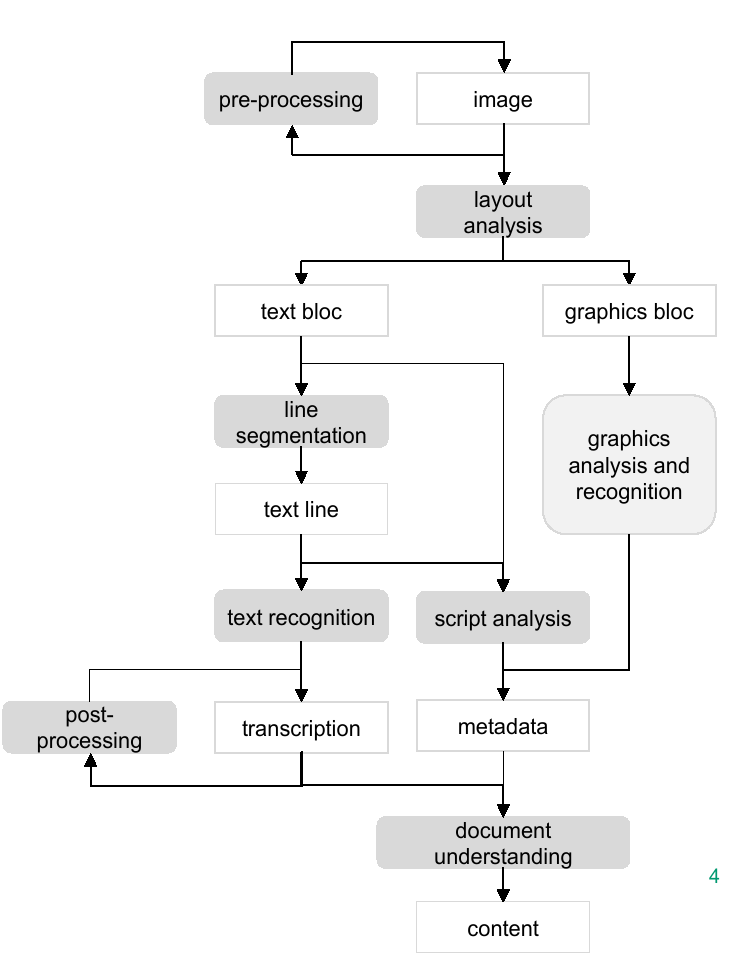
\includegraphics[width=0.5\textwidth]{resources/04_processing_chain}

\subsection{Preprocessing}

Improve quality of images for both visualization as well as processing.
Consists of adjusting resolution, sharpening, colour corrections, deskewing,
binarization, ...

\begin{description}
		\item[Hough transform] skew estimation by mapping pixels to 2D
				parameter space, polar coordinates to estimate skew angle.
		\item[Rotation] can be used to deskew, but introduces distortions
		\item[Bleedthrough] can be removed easily if backside known. Else, use
				gradients.
		\item[Binarization] Global and local operations
\end{description}

\subsection{Layout analysis}

Isolate text blocks, graphics, formula, images, ...

\begin{itemize}
		\item White streams detection recursively does horizontal and vertical
				cuts through white areas. Works well for manhattan layout, less
				well for nested ones. Top-down.
		\item Projectino profiles allow detecting columns or lines, requires
				unskewed image. Top-down.
		\item Connected components, bottom-up aggregation of connected
				components. Useful for binarized printed documents.
		\item Regional classification in e.g. historical documents.
\end{itemize}

\subsection{Text recognition}

\begin{itemize}
		\item OCR suitable for segmented printed text with high-quality images
		\item Handwriting recognition not yet mature, works decently on limited
				vocabulary or when training data available (rather than generic
				model)
		\item Binarization can introduce gaps which lowers OCR performance.
				Context-aware OCR can help, also with similar-looking
				characters.
		\item Sayre's paradox for cursive writing: Character recognition and
				segmentation dependant on each other. Workarounds include
				operations on full words, combining the two, or multiple
				attempts with the most likely one being used.
		\item Depending on alphabet, character recognition (Latin),
				dictionary-based word recognition (Arabic) or stroke
				recognition (Chinese, Japanese) applicable.
\end{itemize}

\subsection{Text alignment}

Align image of text with its transcript. Difficutly depends heavily on accuracy
of transcript and availability of linebreak information.

\subsection{Script analysis}

Script classification, language detection, font recognition, writer
identification, ...

Uses histograms of locale angle distribution, gradients, profiles, run lengths,
...

\subsection{Document understanding}

The last DIA step, first semantic step towards a specific application.
Transformation of physical to logical structure.

\subsubsection{Physical structure}

Publisher's point of view.

\begin{itemize}
		\item Organization of document into regions
		\item Regions into headings and text blocks
		\item Position of figures, separators, ...
\end{itemize}

\subsubsection{Logical structure}

Author's point of view.

\begin{itemize}
		\item Logical structure of document
		\item Articles, titles, headlines, paragraphs, ...
		\item Independent of presentation
\end{itemize}


% No summary for lecture 5 (challenges)
\setcounter{section}{5}

\section{Binary image processing}

\subsection{Binarization}

Goal: Separate foreground and background pixels. Global vs adaptive thresholds.

\subsubsection{Otsu's method}

Minimize threshold of intra-class variance, $p_0 \sigma_0^2 + p_1 \sigma_1^2$,
where $p_i$ is the probability, $\sigma_i^2$ the variance of class $i$.
Equivalent: Maximize inter-class variance $p_0 p_1 (\mu_0 - \mu_1)^2$.

\subsubsection{Niblack's method}

Use local threshold $T_{x, y} = \mu_{x, y} + k \cdot \sigma_{x, y}$, where $k
\in [0, 1]$, typical $k = 0.2$. Window size chosen based on resolution, such
that it contains several characters.

Bad performance if window only includes background!

\subsection{Connected components}

\begin{itemize}
		\item 4-connectivity: Orthogonally connected pixels
		\item 8-connectivity: All neighbouring pixels
		\item n-connected path: Path connected via n-connectivity. E.g.
				4-connected path is akin to movement in Snake, 8-connected path
				akin to movement of queen in chess.
		\item n-connected component IFF for every pair of pixels, there is an
				n-connected path connecting them.
\end{itemize}

\subsection{Jordan's theorem}

In continuous space, a closed simple curve divides the plane into two connected
regions.

In discrete space, a 4-connected curve delimits two 8-connected regions, a
8-connected curve delimits two 4-connected regions.

\subsection{Extracting connected components}

\subsubsection{2D scanning}

Suitable for many small components. Works by only comparing black runs on
current line to those in previous lines. Builds up compoments, merging where
applicable.

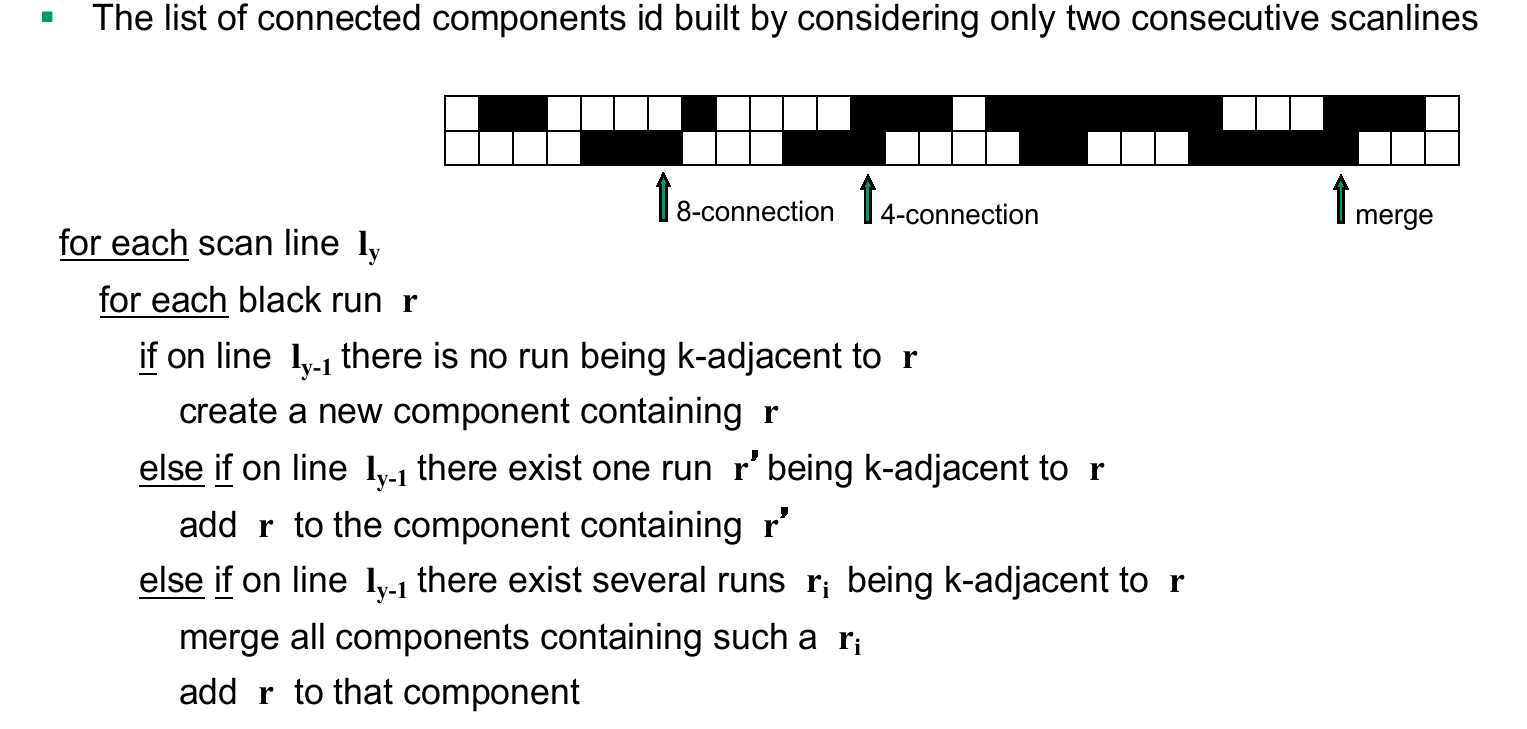
\includegraphics[width=0.5\textwidth]{06_2d_scanning}

\subsubsection{Border following algorithm}

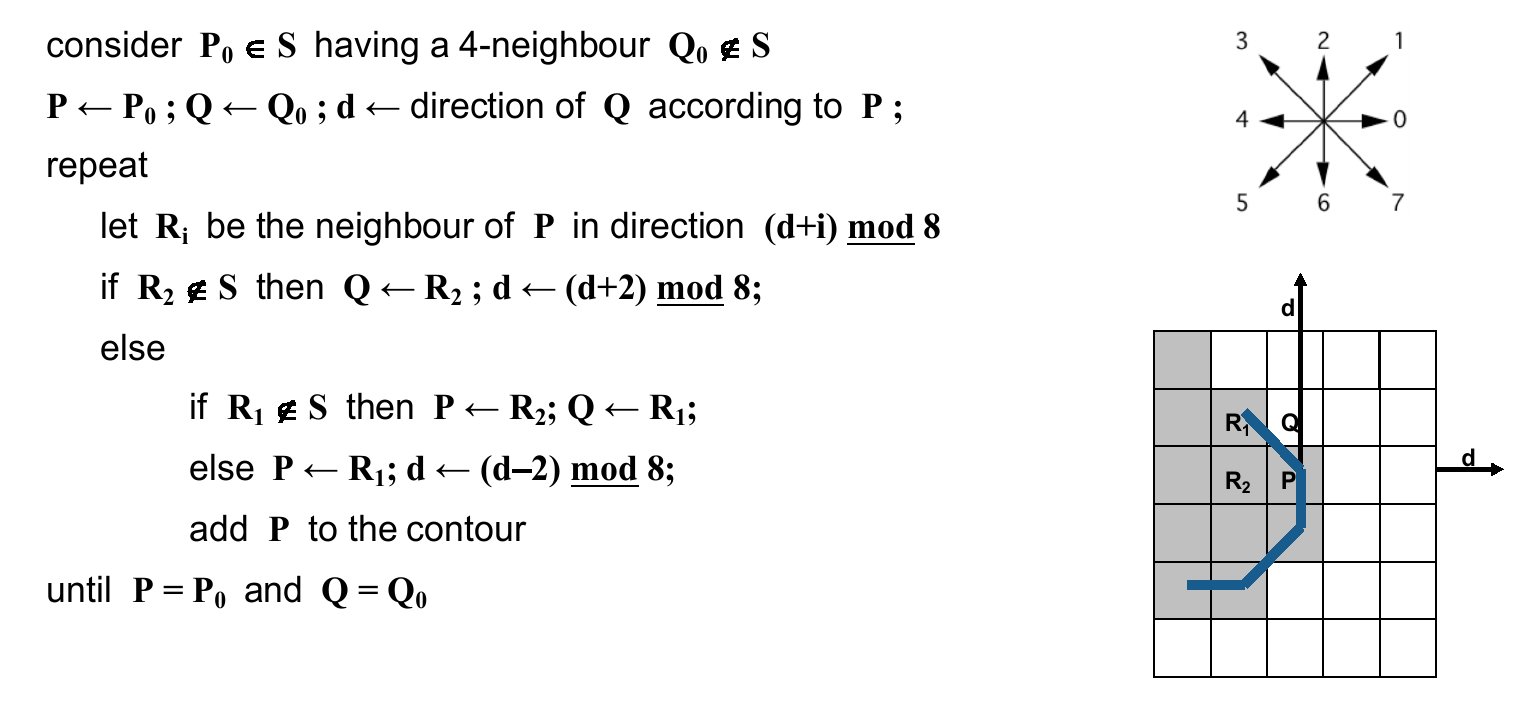
\includegraphics[width=0.5\textwidth]{06_border}

\subsection{Morphological operations}

Operations using a mask (`structurnig element') and an operation, to modify
pixel based on its neighbours. (Local operation).

\subsubsection{Erosion}

Idea: Keep pixels where every pixel of mask has a corresponding pixel on image.
Example mask: Cross shape.

$X \Theta M = \{p | M_p \subset X\}$

\subsubsection{Dilation}

Keep pixels for which any pixel of mask overlaps the shape.

$X \oplus M = \{p | M_p \cap X \neq \emptyset\}$

\subsubsection{Duality of erosion and dilation}

Erosion of inverse is inverse of dilation, and dilation of inverse is inverse
of dilation.

\begin{align*}
		\bar{X} \Theta M = \bar{X \oplus M} \\
		\bar{X} \oplus M = \bar{X \Theta M}
\end{align*}

\subsubsection{Opening and closing}

Let $M^{-}$ be the `symmetric' (mirrored along anchor point) structural
element. If $M$ is symmetric, $M = M^{-}$.

\paragraph{Opening}

Erasion then dilation.

\[
		X \circ M = (X \Theta M) \oplus M^{-}
\]

\paragraph{Closing}

Dilation then erosion.

\[
		X \bullet M = (X \oplus M) \Theta M^{-}
\]

\paragraph{Properties}

\begin{align*}
		\bar{X} \circ M = \bar{X \bullet M}, \bar{X} \bullet M = \bar{X \circ M} && \text{Duality} \\
		X \circ M \subset X, X \subset X \bullet M && \text{Opening is subset, closing is superset of image} \\
		X \subset Y \Rightarrow (X \circ M) \subset (Y \circ M), (X \bullet M) \subset (Y \bullet M) && \text{Monotonically increasing} \\
		(X \circ M) \circ M = X \circ M, (X \bullet M) \bullet M = X \bullet M && \text{Idempotent} \\
		(X \circ M) = \cup \{M_p | M_p \subset X\}
\end{align*}

\subsubsection{Run-length smoothing}

Widely used technique for layout analysis, fill white gaps below a given
threshold horizontally or verticall. Corresponds to opening with $1 \times T$
mask.

\subsubsection{Hit and miss operator}

\[
		\operatorname{ham}_{M_0, M_1}(X) = X \otimes (M_0, M_1) = (X \Theta M_1) \cap (\bar{X} \theta M_0)
\]

Hit and miss operator can be represented as one ternary (three-valued) mask,
where the mask is black where masks one is $1$, white where mask two is $1$,
gray where both masks are white.

\subsubsection{Thinning}

\[
		\operatorname{thin}_M(X) = X - \operatorname{ham}_M(X) = X \cap \bar{(\operatorname{ham}_M(X))}
\]

\subsubsection{Homotopic transformation}

A transformation is homotopic IFF the connexity of all components is preserved,
including wholes. Compare e.g. standard erosion: Can break up components, so is
not homotopic.

Operations can be made homotopic by using special masks.

\subsubsection{Skeleton in euclidean and discrete geometry}

Skeleton $\operatorname{skel}(X)$ of connected component $X$ is all points in
the canters of the maximal inscribed circles. No satisfying of this definition
in discrete space however.

Discrete skeletonization achieved with iterative homotopic transformations,
converting a connected component $X$ into skinny curves.

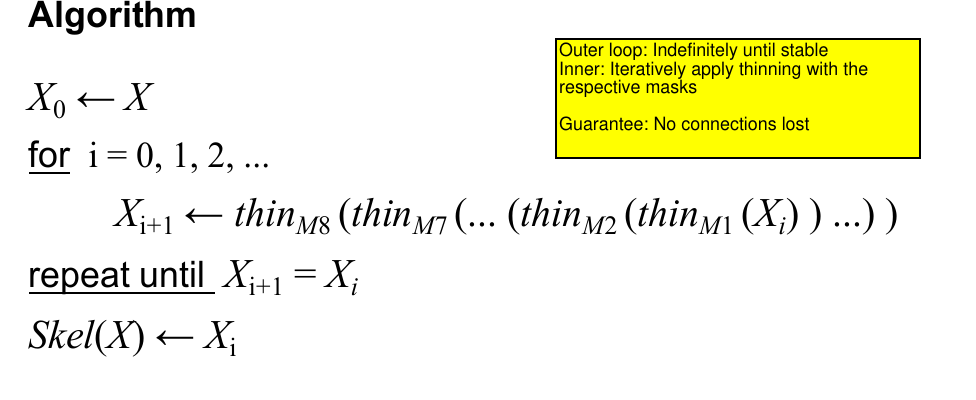
\includegraphics[width=0.5\textwidth]{06_skeletonization}

\subsubsection{Pruning}

Can be used to remove separated pixels after skeletonization. Removes terminal
pixels via hit and miss using certain masks.


\section{Text recognition}

Goal: Transcription (ASCII or Unicode) of text. Analysis also covers language
and script recognition, font recognition, writer authentication, word spotting,
...

OCR good results for non-cursive printed text, clean images, high resolution.
Challenging for cursive script, continuous handwritten text, degraded
documents.

\subsection{Sayre's paradox}

With cursive text / connected characters, character recognition requires
character segmentation, and character segmentation requires character
recognition. Approaches: Recognize whole worlds, test multiple hypothesis,
combine the two.

\subsection{Processing steps}

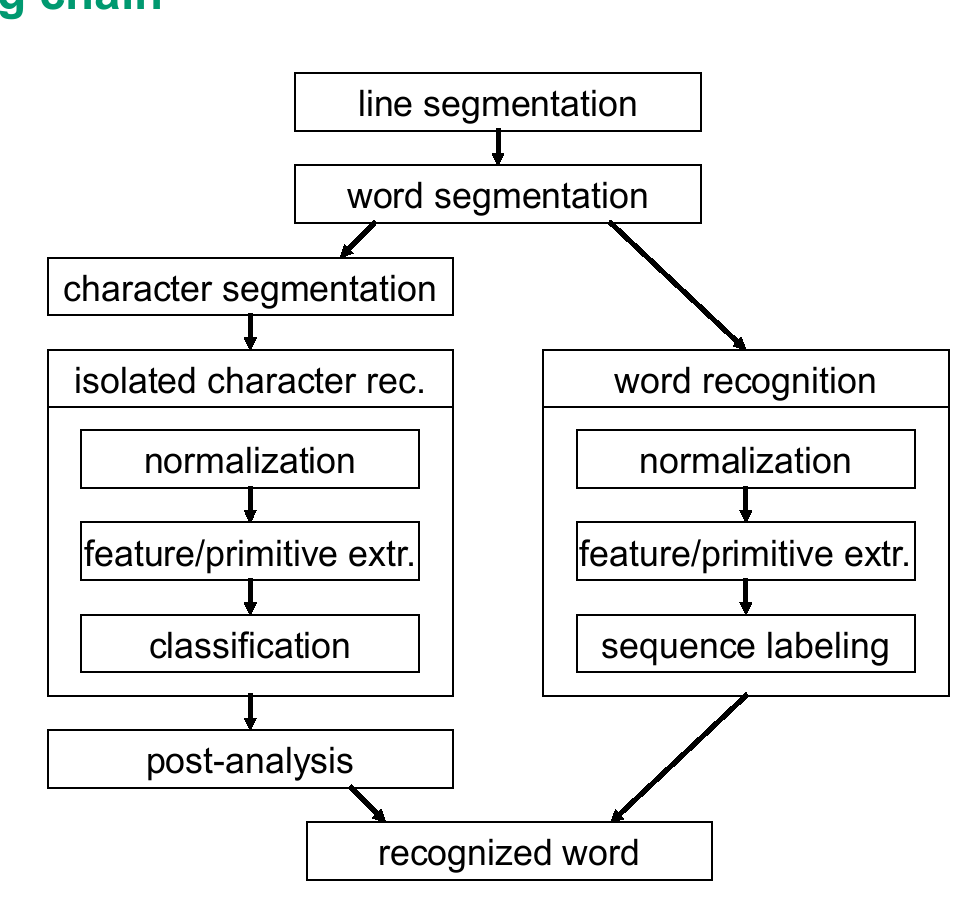
\includegraphics[width=0.5\textwidth]{07_processing}

\subsection{Character recognition}

\begin{itemize}
		\item Isolated character recognition applicable to high-quality printed
				text or constrained handwriting. Challenge: Variability of
				class.
		\item Classification: Statistical (KNN, SVM, ...), direct comparison
				with model, pattern recognition
		\item Similarity measures: Hamming distance, warping distance
		\item Two steps: Feature extraction, then classification
		\item Typical features: Dimensions, density, projection profiles, HOG,
				LBP, ...
\end{itemize}

\subsubsection{Structural approaches}

\begin{itemize}
		\item Shapes decomposed into strokes, properties extracted: Number of
				connected components, number of holes, concavities and
				convexities, ...
		\item These primitives represented as strings, trees, graphs and compared
\end{itemize}

\subsection{Classification}

\begin{description}
		\item[KNN] Sample classified by plurality vote of its neighbours (see
				which class majority of its $k$ nearest neighbours belong to)
		\item[MLP] Fully connected neural network with hidden layer, decision
				based on highest activation on output layer
		\item[SVM] Map initial feature space to augmented space where linear
				discrimination possible. Finds hyperplane with maximum
				separating distance between classes.
\end{description}

\subsection{Word recognition}

\begin{itemize}
		\item Alternative to character recognition, useful if limited
				vocabulary, language-driven approach or keyword spotting
		\item Typically used for cursive scripts, handwriting or
				difficult-to-segment scripts
		\item More possible cases, more features needed
		\item But can use external language knowledge, dictionaries, ...
		\item Feature extraction using sliding window
		\item Dynamic time warping, hidden markov models, ... suitable for
				sequential data analysis
\end{itemize}

\subsubsection{Dynamic time warping}

\begin{itemize}
		\item Calculates similarity between time series, based on DP
\end{itemize}

\subsubsection{Hidden markov model}

\begin{itemize}
		\item Class modeled by a two-stage stochastic process using hidden and
				visible state.
		\item Hidden model has states and transition function (think FSM).
				Observations linked to states via emission functions. Idea:
				Predict state via observations.
		\item That is pick state which best explains patterns in observations.
\end{itemize}


\section{Deep learning}

\begin{itemize}
		\item Machine learning: Decisions determined by a model trained on data
		\item Deep learning: Machine learning based on neural networks
		\item Historically not applicable because of vanishing gradient problem
				(slow convergence), but recent progress due to better
				algorithms, increased processing power and large datasets
\end{itemize}

\subsection{Perceptron}

\begin{itemize}
		\item Calculates weighted sum of inputs
		\item Bias to shift value
		\item Non-linear activation function determines whether output activates or not
\end{itemize}

\[
		\hat{y} = g (w_0 + \sum_{i = 1}^m x_i w_i)
\]

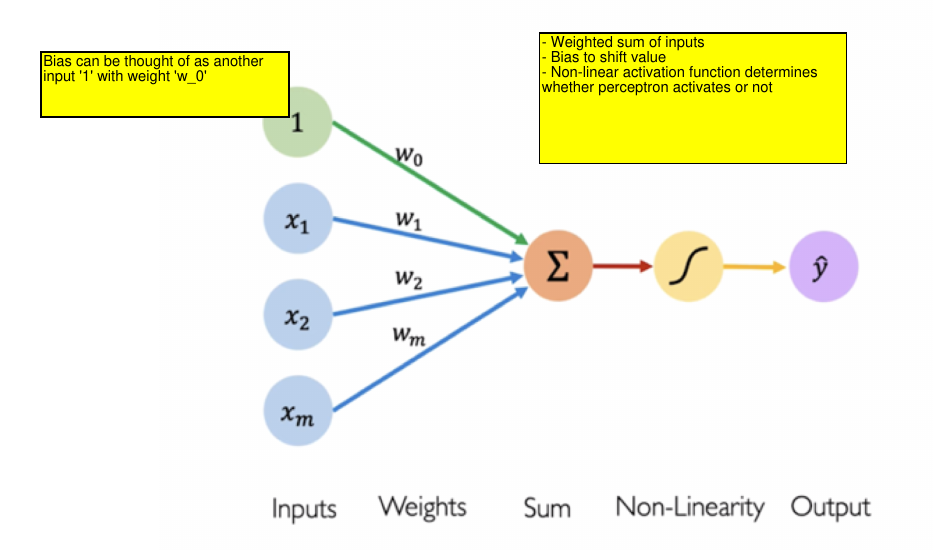
\includegraphics[width=0.7\textwidth]{08_perceptron}

\subsubsection{Common activation functions}

\paragraph{Sigmoid function}

\begin{align*}
		g(z) & = \frac{1}{1 + e^{-z}} \\
		g'(z) & = g(z) \cdot (1 - g(z))
\end{align*}

\paragraph{Hyperbolic tangent}

\begin{align*}
		g(z) & = \frac{e^z - e^{-z}}{e^z + e^{-z}} \\
		g'(z) & = 1 - g(z)^2
\end{align*}

\paragraph{Rectified linear unit}

\begin{align*}
		g(z) & = \max(0, z) \\
		g'(z) & = \left\{\begin{array}{lr}
						1, & \text{for } z > 0 \\
						0, & \text{otherwise} \\
		\end{array}\right.
\end{align*}

\subsection{Single layer neural network}

\begin{itemize}
		\item One hidden layer of perceptrons
		\item Fully connected
		\item One weight matrix per perceptron (with one weight per input each) for input -> hidden transition
		\item And one weight matrix per perceptron for hidden -> output transition
		\item Final outputs are then weighted sums of each perceptron's output,
				again with a weight per perceptron / final output pair, fed
				once more through non-linear activation function.
				\begin{itemize}
						\item Final outputs are effectively perceptrons too,
								which use hidden layer as inputs.
				\end{itemize}
\end{itemize}

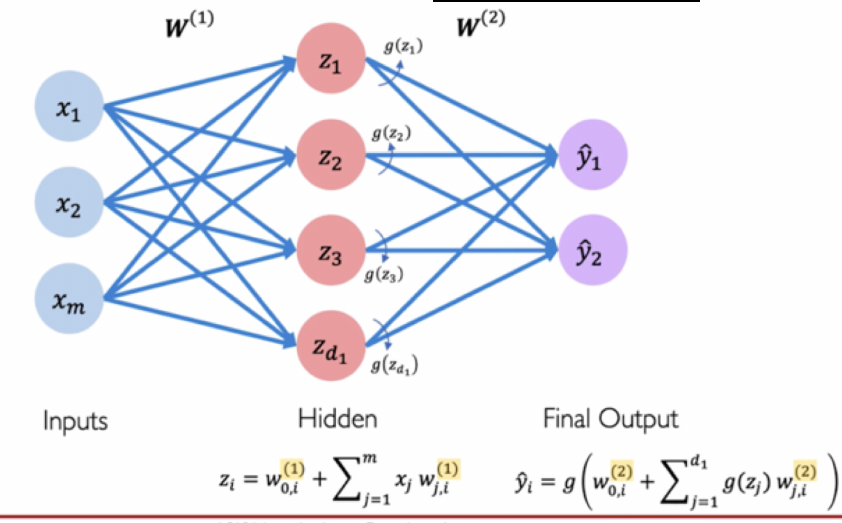
\includegraphics[width=0.7\textwidth]{08_single_layer}

\subsection{Deep neural network}

\begin{itemize}
		\item Many (in practice: several hundred) hidden layers, each consuming
				outputs of previous layer.
\end{itemize}

\subsection{Empirical loss}

\begin{itemize}
		\item Measures total loss over dataset.
		\item `Cost' incurred to network if predicted output incorrect, used to
				train network by making it minimize loss.
		\item During training, network finds weights such as to minimize loss.
\end{itemize}

\begin{align*}
		J(W) = \frac{1}{n} \sum_{i = 1}^n L(f(x^{(i)}; W), y^{(i)})
\end{align*}

Where $x$ inputs, $y$ labels, $f(x)$ predictions, $W = \{W^{(i)}$ weights,
		$J(W)$ total loss, $L()$ loss function, $f(x^{(i)}; W)$ predicted given
		set of weights.

\subsection{Loss optimization}

Find weights $W*$ which achieve lowest loss:

\begin{align*}
		W* = \operatorname{argmin}_W J(W)
\end{align*}

\subsection{Gradient descent}

Move along `down' direction in multidimensional space until convergence.

\subsubsection{Backpropagation}

Problem: How to figure out how to change weights to go `down'? Idea: Use chain
rule to recursively figure out effect changes to weight will have on loss.

Example: Shows how changes to $w_1$ will affect final loss.

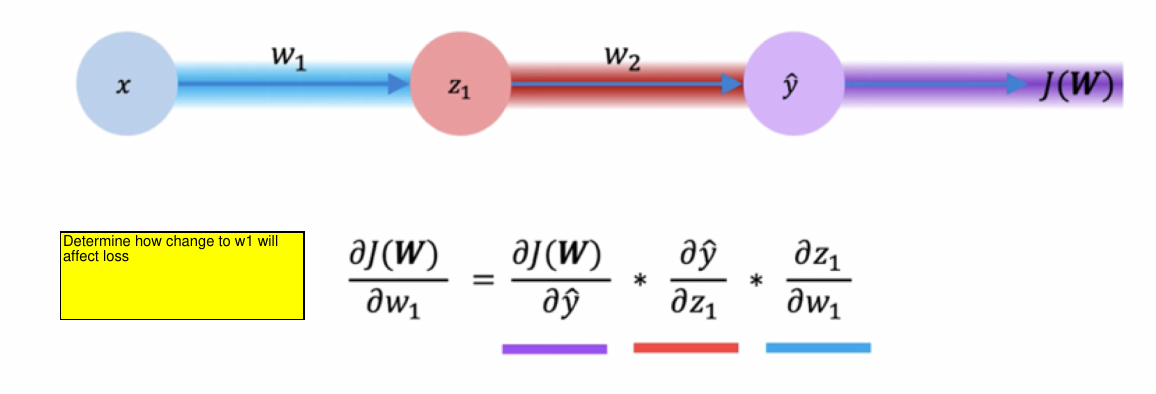
\includegraphics[width=0.7\textwidth]{08_backpropagation}

\subsubsection{Gradient descent algorithm}

\begin{enumerate}
		\item Initialize weights randomly with normal distribution around $0$
		\item Loop until convergence:
				\begin{enumerate}
						\item Compue gradient $\frac{\partial J(W)}{\partial W}$
						\item Update weights $W \coloneqq W - \eta
								\frac{\partial J(W)}{\partial W}$ with learning
								rate $\eta$
				\end{enumerate}
		\item Return weights
\end{enumerate}

\subsubsection{Stochastic gradient descent}

To accelerate convergence: Instead of calculating gradient over full dataset
(costly), use random batch $B$ (order 10s - 100s) over which to calculate
gradient:

\begin{align*}
		\frac{\partial J(W)}{\partial W} = \frac{1}{B} \sum_{k = 1}^B \frac{\partial J_k(W)}{\partial W}
\end{align*}

\subsubsection{Avoiding local minima}

\begin{itemize}
		\item Repeat training with multiple initializations
		\item Adapt learning rates. Too low has risk of being stuck in local
				minima, too high has risk of overshooting.
		\item Less risk of local minima in higher-dimensional spaces.
\end{itemize}

\subsection{Avoiding over-fitting}

\begin{itemize}
		\itemize Dropout: Randomly set certain weights per layer to 0, prevent
				network from becoming too complex
		\item Early stopping: Separate validation set, stop training once
				validation set minimized loss
\end{itemize}


\clearpage

\end{document}

